\documentclass[12pt]{article}
\usepackage{dsfont}
\usepackage{textcomp}
\usepackage{amsmath}
\usepackage{amssymb}
\usepackage{graphicx}
\usepackage{array}


\begin{document}


\title{Solutions to Sheet 11}
\author{Lukas Drexler, Leif Van Holland \\ \\
\textsc{Pattern Matching and Machine Learning} \\
\textsc{for Audio Signal Processing}}
\maketitle

\section*{Exercise 11.1}
\begin{itemize}
    \item[a)]
    Given $X=(1,7,4,4,6)$ and $Y=(1,2,2,7)$, we get
    \[ C=
    \begin{pmatrix}
        0 & 1 & 1 & 6 \\
        6 & 5 & 5 & 0 \\
        3 & 2 & 2 & 3 \\
        3 & 2 & 2 & 3 \\
        5 & 4 & 4 & 1
    \end{pmatrix}, \quad D = 
    \begin{pmatrix}
        0 & 1 & 2 & 8 \\
        6 & 6 & 6 & 2 \\
        9 & 8 & 8 & 5 \\
        12 & 10 & 10 & 8 \\
        17 & 14 & 14 & 9
    \end{pmatrix}
    \]
    From $D$, we can easily find the one optimal path
    \[p = ((5,4),(4,4),(3,4),(2,4),(1,3),(1,2),(1,1)). \]
    \item[b)]
    Now given $X=(1,2,2,1)$ and $Y=(1,0,0,1)$ we can again calculate the matrices
    \[ C=
    \begin{pmatrix}
        0 & 1 & 1 & 0 \\
        1 & 2 & 2 & 1 \\
        1 & 2 & 2 & 1 \\
        0 & 1 & 1 & 0
    \end{pmatrix}, \quad D = 
    \begin{pmatrix}
        0 & 1 & 2 & 2 \\
        1 & 2 & 3 & 3 \\
        2 & 3 & 4 & 4 \\
        2 & 3 & 4 & 4
    \end{pmatrix}
    \]
    This time, we find the following 7 optimal paths:
    \begin{align*}
        q_1 &= ((4,4),(3,4),(2,4),(1,4),(1,3),(1,2),(1,1)) \\
        q_2 &= ((4,4),(3,4),(2,4),(1,3),(1,2),(1,1)) \\
        q_3 &= ((4,4),(3,4),(2,3),(1,2),(1,1)) \\
        q_4 &= ((4,4),(3,3),(2,2),(1,1)) \\
        q_5 &= ((4,4),(4,3),(3,2),(2,1),(1,1)) \\
        q_6 &= ((4,4),(4,3),(4,2),(3,1),(2,1),(1,1)) \\
        q_7 &= ((4,4),(4,3),(4,2),(4,1),(3,1),(2,1),(1,1)) \\
    \end{align*}
\end{itemize}

\section*{Exercise 11.2}

\begin{center}
    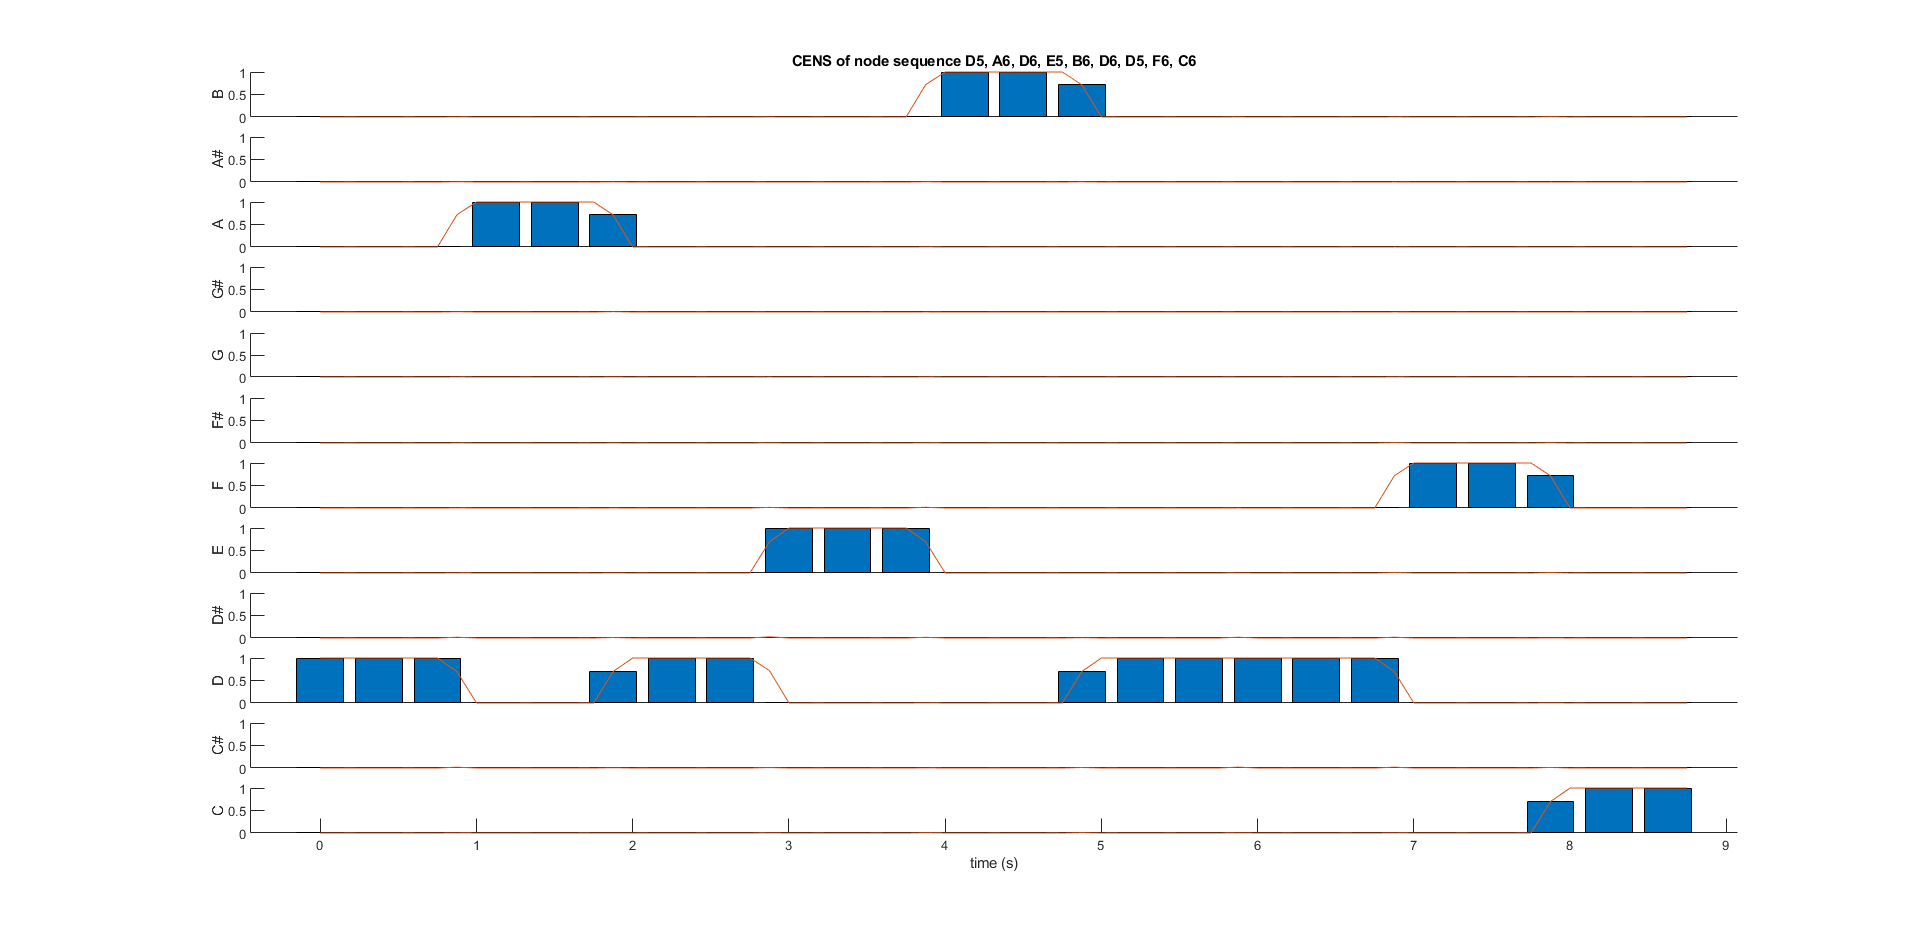
\includegraphics[width=\textwidth]{cens}
\end{center}

\end{document}
